\usetikzlibrary{shapes.geometric}
\usetikzlibrary{arrows.meta}
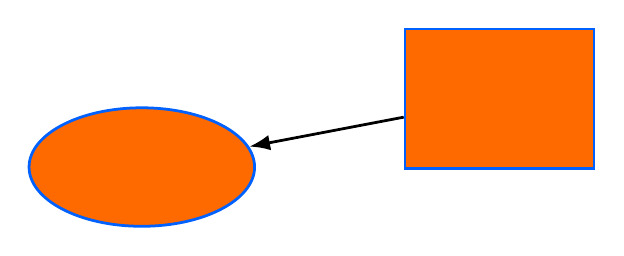
\begin{tikzpicture}

    
    \node[rectangle, minimum width=2.399cm, minimum height=1.775cm, draw={rgb,255:red,0;green,97;blue,254}, fill={rgb,255:red,255;green,106;blue,0}, text={rgb,255:red,0;green,0;blue,0}, line width=1pt] (ndNode2) at (9.484,7.067) {};
    \node[draw={rgb,255:red,0;green,97;blue,254}, fill={rgb,255:red,255;green,106;blue,0}, text={rgb,255:red,0;green,0;blue,0}, line width=1pt, ellipse, minimum width=2.864cm, minimum height=1.505cm] (ndNode3) at (4.941,6.202) {};
    \draw[draw={rgb,255:red,0;green,0;blue,0}, line width=1pt, -{Latex}] (ndNode2) -- (ndNode3);
\end{tikzpicture}
